% Options for packages loaded elsewhere
\PassOptionsToPackage{unicode}{hyperref}
\PassOptionsToPackage{hyphens}{url}
\PassOptionsToPackage{dvipsnames,svgnames,x11names}{xcolor}
%
\documentclass[
  letterpaper,
  DIV=11,
  numbers=noendperiod]{scrartcl}

\usepackage{amsmath,amssymb}
\usepackage{iftex}
\ifPDFTeX
  \usepackage[T1]{fontenc}
  \usepackage[utf8]{inputenc}
  \usepackage{textcomp} % provide euro and other symbols
\else % if luatex or xetex
  \usepackage{unicode-math}
  \defaultfontfeatures{Scale=MatchLowercase}
  \defaultfontfeatures[\rmfamily]{Ligatures=TeX,Scale=1}
\fi
\usepackage{lmodern}
\ifPDFTeX\else  
    % xetex/luatex font selection
\fi
% Use upquote if available, for straight quotes in verbatim environments
\IfFileExists{upquote.sty}{\usepackage{upquote}}{}
\IfFileExists{microtype.sty}{% use microtype if available
  \usepackage[]{microtype}
  \UseMicrotypeSet[protrusion]{basicmath} % disable protrusion for tt fonts
}{}
\makeatletter
\@ifundefined{KOMAClassName}{% if non-KOMA class
  \IfFileExists{parskip.sty}{%
    \usepackage{parskip}
  }{% else
    \setlength{\parindent}{0pt}
    \setlength{\parskip}{6pt plus 2pt minus 1pt}}
}{% if KOMA class
  \KOMAoptions{parskip=half}}
\makeatother
\usepackage{xcolor}
\setlength{\emergencystretch}{3em} % prevent overfull lines
\setcounter{secnumdepth}{-\maxdimen} % remove section numbering
% Make \paragraph and \subparagraph free-standing
\ifx\paragraph\undefined\else
  \let\oldparagraph\paragraph
  \renewcommand{\paragraph}[1]{\oldparagraph{#1}\mbox{}}
\fi
\ifx\subparagraph\undefined\else
  \let\oldsubparagraph\subparagraph
  \renewcommand{\subparagraph}[1]{\oldsubparagraph{#1}\mbox{}}
\fi


\providecommand{\tightlist}{%
  \setlength{\itemsep}{0pt}\setlength{\parskip}{0pt}}\usepackage{longtable,booktabs,array}
\usepackage{calc} % for calculating minipage widths
% Correct order of tables after \paragraph or \subparagraph
\usepackage{etoolbox}
\makeatletter
\patchcmd\longtable{\par}{\if@noskipsec\mbox{}\fi\par}{}{}
\makeatother
% Allow footnotes in longtable head/foot
\IfFileExists{footnotehyper.sty}{\usepackage{footnotehyper}}{\usepackage{footnote}}
\makesavenoteenv{longtable}
\usepackage{graphicx}
\makeatletter
\def\maxwidth{\ifdim\Gin@nat@width>\linewidth\linewidth\else\Gin@nat@width\fi}
\def\maxheight{\ifdim\Gin@nat@height>\textheight\textheight\else\Gin@nat@height\fi}
\makeatother
% Scale images if necessary, so that they will not overflow the page
% margins by default, and it is still possible to overwrite the defaults
% using explicit options in \includegraphics[width, height, ...]{}
\setkeys{Gin}{width=\maxwidth,height=\maxheight,keepaspectratio}
% Set default figure placement to htbp
\makeatletter
\def\fps@figure{htbp}
\makeatother
\newlength{\cslhangindent}
\setlength{\cslhangindent}{1.5em}
\newlength{\csllabelwidth}
\setlength{\csllabelwidth}{3em}
\newlength{\cslentryspacingunit} % times entry-spacing
\setlength{\cslentryspacingunit}{\parskip}
\newenvironment{CSLReferences}[2] % #1 hanging-ident, #2 entry spacing
 {% don't indent paragraphs
  \setlength{\parindent}{0pt}
  % turn on hanging indent if param 1 is 1
  \ifodd #1
  \let\oldpar\par
  \def\par{\hangindent=\cslhangindent\oldpar}
  \fi
  % set entry spacing
  \setlength{\parskip}{#2\cslentryspacingunit}
 }%
 {}
\usepackage{calc}
\newcommand{\CSLBlock}[1]{#1\hfill\break}
\newcommand{\CSLLeftMargin}[1]{\parbox[t]{\csllabelwidth}{#1}}
\newcommand{\CSLRightInline}[1]{\parbox[t]{\linewidth - \csllabelwidth}{#1}\break}
\newcommand{\CSLIndent}[1]{\hspace{\cslhangindent}#1}

\KOMAoption{captions}{tableheading}
\makeatletter
\makeatother
\makeatletter
\makeatother
\makeatletter
\@ifpackageloaded{caption}{}{\usepackage{caption}}
\AtBeginDocument{%
\ifdefined\contentsname
  \renewcommand*\contentsname{Table of contents}
\else
  \newcommand\contentsname{Table of contents}
\fi
\ifdefined\listfigurename
  \renewcommand*\listfigurename{List of Figures}
\else
  \newcommand\listfigurename{List of Figures}
\fi
\ifdefined\listtablename
  \renewcommand*\listtablename{List of Tables}
\else
  \newcommand\listtablename{List of Tables}
\fi
\ifdefined\figurename
  \renewcommand*\figurename{Figure}
\else
  \newcommand\figurename{Figure}
\fi
\ifdefined\tablename
  \renewcommand*\tablename{Table}
\else
  \newcommand\tablename{Table}
\fi
}
\@ifpackageloaded{float}{}{\usepackage{float}}
\floatstyle{ruled}
\@ifundefined{c@chapter}{\newfloat{codelisting}{h}{lop}}{\newfloat{codelisting}{h}{lop}[chapter]}
\floatname{codelisting}{Listing}
\newcommand*\listoflistings{\listof{codelisting}{List of Listings}}
\makeatother
\makeatletter
\@ifpackageloaded{caption}{}{\usepackage{caption}}
\@ifpackageloaded{subcaption}{}{\usepackage{subcaption}}
\makeatother
\makeatletter
\@ifpackageloaded{tcolorbox}{}{\usepackage[skins,breakable]{tcolorbox}}
\makeatother
\makeatletter
\@ifundefined{shadecolor}{\definecolor{shadecolor}{rgb}{.97, .97, .97}}
\makeatother
\makeatletter
\makeatother
\makeatletter
\makeatother
\ifLuaTeX
  \usepackage{selnolig}  % disable illegal ligatures
\fi
\IfFileExists{bookmark.sty}{\usepackage{bookmark}}{\usepackage{hyperref}}
\IfFileExists{xurl.sty}{\usepackage{xurl}}{} % add URL line breaks if available
\urlstyle{same} % disable monospaced font for URLs
\hypersetup{
  pdftitle={A Time Series Approach to Modeling Potential Solar Output},
  pdfauthor={Nathaniel Reimer, Kyle Suelflow},
  colorlinks=true,
  linkcolor={blue},
  filecolor={Maroon},
  citecolor={Blue},
  urlcolor={Blue},
  pdfcreator={LaTeX via pandoc}}

\title{A Time Series Approach to Modeling Potential Solar Output}
\author{Nathaniel Reimer, Kyle Suelflow}
\date{2023-12-19}

\begin{document}
\maketitle
\begin{abstract}
Replacing carbon-emitting energy sources with greener alternatives is
critical to preventing worst-case climate change scenarios. Solar power
is an incredible option. To make the best use of solar power, we need to
have a way to model potential solar output over long and short periods.
We use time-series methods to model Global Horizontal Irradiance (GHI)
at the hourly and daily levels. Using a sine function to model hourly
GHI, we find a correlation between data taken less than four hours
apart. After removing multiple seasonal relationships in the aggregated
daily data, we find a correlation between data two to three days apart.
We also show that each location we modeled required unique
considerations and approaches.
\end{abstract}
\ifdefined\Shaded\renewenvironment{Shaded}{\begin{tcolorbox}[sharp corners, breakable, boxrule=0pt, interior hidden, frame hidden, borderline west={3pt}{0pt}{shadecolor}, enhanced]}{\end{tcolorbox}}\fi

\hypertarget{introduction}{%
\subsection{Introduction}\label{introduction}}

Greenhouse gas emissions have exploded in recent decades, causing
substantial damage to the livelihoods of many across the world. One of
the main culprits of these emissions is the energy sector. Using
non-renewables such as Coal, Oil, and natural gas to create electricity
causes carbon and other GHGs to be emitted. To combat this, renewable
energy has been brought forward as the leading solution to this crisis.
Solar and wind energy, specifically, have the most potential to create
lasting change in regards to our energy usage. The reality of this
situation has brought us to think about modeling different solar
variables. Being able to model Global Horizontal Irradiance, for
example, allows places around the globe to gain a better understanding
of whether or not they would be suitable for solar energy. Qualitative
measures such as economic feasibility, the physical geography of places,
and political and regulatory hurdles are other things that places can
take into account in order to determine if solar is feasible for them,
in addition to considering this analysis (Crook et al. 2011; Wild,
Folini, and Henschel 2017; Boland 2020; Shahsavari and Akbari 2018).
This leads us into our two research questions:

\begin{itemize}
\tightlist
\item
  How well can we model Global Horizontal Irradiance using a time series
  approach for different situations across the world? And,
\item
  Are the models we create consistent across the 25 year period
  (1998-2023) for which we have data from?
\end{itemize}

\hypertarget{data-context}{%
\subsubsection{Data Context}\label{data-context}}

This project focuses on Global Horizontal Irradiance (GHI), a measure of
the power of the power of sunlight that reaches the horizontal ground
(Stein, Hansen, and Reno 2012). GHI can then be used to estimate the
output of a hypothetical solar installation placed on the ground. GHI
data used in this report is part of a publicly available GHI data set
from SolarAnywhere. SolarAnywhere uses data from geosynchronous
satellites to estimate GHI rather than measuring it directly with ground
stations ({``Historical Data Validation''} 2023). Their model is
calibrated with data from ground stations. Annual data is accurate
within \(\pm\) 4.2\% based on this validation. Errors increase for
shorter time periods: monthly data has an RMSE of 3.9\% and hourly data
has an RMSE of 20.6\%.

We focus our analysis on Victoria, Seychelles, with comparisons to
Nairobi, Kenya, and Manchester, England. Nairobi and Victoria are at
similar latitudes and so receive a similar amount of sun throughout the
year but have different climates. Manchester's sunlight is more seasonal
because of its latitude and it has a very different climate.

We use daily Solar Insolation data in our analysis of daily GHI. Solar
Insolation in our data is the amount of downward solar energy incident
at the top of the atmosphere (Hartmann 2016). It varies by latitude and
time of year. We generate daily insolation data for each of our selected
locations using the Python package climlab (Rose et al. 2022). The
insolation data has units of \(\frac{W}{m^2}\) per hour. Hourly GHI data
has also has units of \(\frac{W}{m^2}\) per hour. The difference is that
GHI is measured on the ground and solar insolation is measured at the
top of the atmosphere.

\hypertarget{model-discussion-and-justification}{%
\subsection{Model Discussion and
Justification}\label{model-discussion-and-justification}}

\hypertarget{intra-day-variation-in-ghi}{%
\subsubsection{Intra-Day Variation in
GHI}\label{intra-day-variation-in-ghi}}

To begin, we wanted to model the intra-day variation in GHI across our
sites, and across the 25 year period. An overview of the process is as
follows: First, we found the best fitting sine curve to model the
average GHI by month for a given 5-year period. Next, we extrapolated
this curve onto the plot of ALL data points (no longer mean GHI, but
GHI). Then, we used a GEE model to model the residuals of our sine curve
model, which determined what order AR model to use. We used five
different 5-year periods in order to see if there was any changes in our
model across time. For the purposes of this explanation, we will show
what the process looked like for the years 1998-2002 across each of our
three locations.

For the first step of our process, we decided to model GHI throughout a
day by using a sine curve. We made this choice based on striking
similarities between the shape of our distribution and that of a sine
curve. The equation for the sine curve we chose is listed below:
\(curveFit = \sin(\pi(time - P)/24)\) \texttt{time} is an integer
measured from 0 to 24, representing an hour of a given day. \texttt{P}
is a parameter used to phase shift the sine curve left or right. This
equation is consistent across all three locations except for \texttt{P}.
We put the results of \texttt{curveFit} into the linear model below:
\(MeanGHI \sim curveFit*Night*factor(Month)\)

where \texttt{Month} is a categorical variable for the month of the year
and \texttt{Night} is an indicator variable that says whether or not it
is nighttime, i.e.~the GHI is zero. \texttt{Night} is coded differently
for each location. For the Seychelles, since it's latitude is only 4
degrees south of the equator, it did not have much variation in terms of
the length of daylight during a day. As such, \texttt{Night} could be
thought of as between 8 in the morning and 6 at night. For Nairobi,
since it's latitude is very similar to Seychelles', we treated
\texttt{Night} the same. But, for Manchester, as it's latitude is 53
degrees north of the equator, the length of daytime throughout the year
changes drastically. Thus, we changed how we coded \texttt{Night}. For
Manchester, if the minimimum GHI for a given month at a given hour is 0,
meaning that at least once during a month the GHI is zero at that hour,
then we treated that hour as Nighttime. You can see the variation, or
lack thereof, in GHI during a day for each month below. Nairobi is
pretty similar to Seychelles, and thus is not shown.

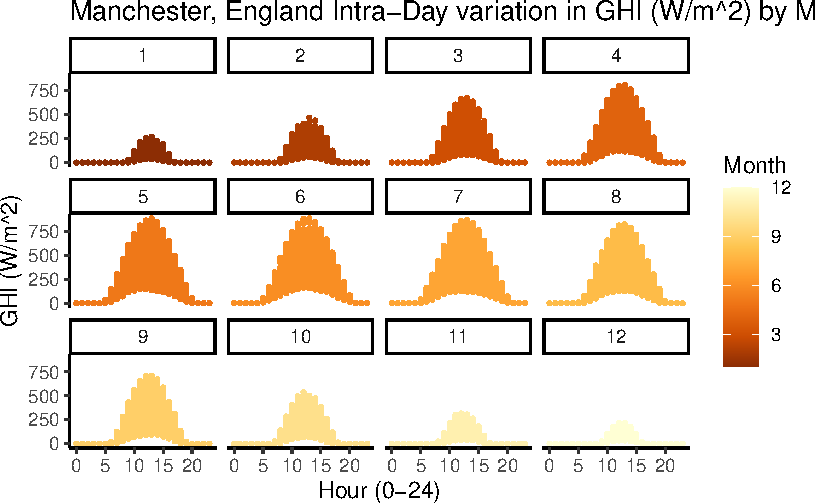
\includegraphics{FinalReport_files/figure-pdf/unnamed-chunk-1-1.pdf}

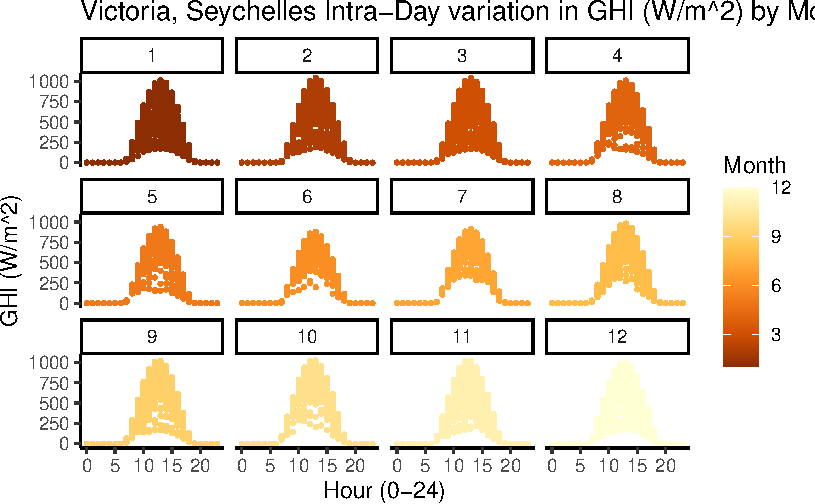
\includegraphics{FinalReport_files/figure-pdf/unnamed-chunk-1-2.pdf}

To determine phase shift parameter for each location, we found the
optimal parameter based on the minimum of the sum of the squared
residuals.

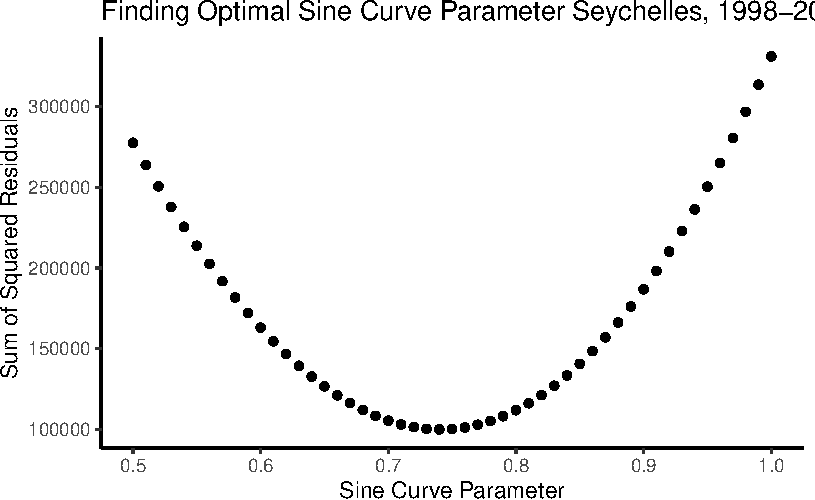
\includegraphics{FinalReport_files/figure-pdf/finding sine parameter Seychelles-1.pdf}

Based on this scatterplot, we chose a parameter of 0.74 for Victoria
Seychelles. Similar plots were done for Nairobi and Manchester,
producing a parameter of 1.07 and 0.56, respectively. Now that we have
an optimized sine curve model, we fit the to model GHI against hour
within the day.

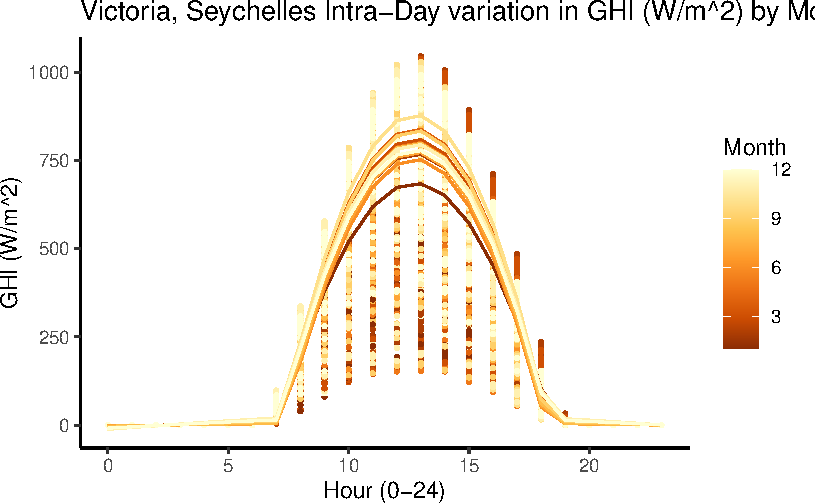
\includegraphics{FinalReport_files/figure-pdf/unnamed-chunk-3-1.pdf}

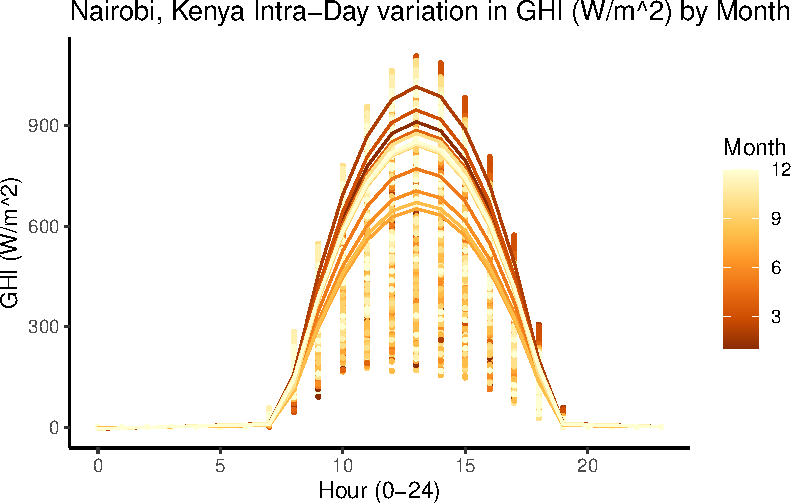
\includegraphics{FinalReport_files/figure-pdf/unnamed-chunk-4-1.pdf}

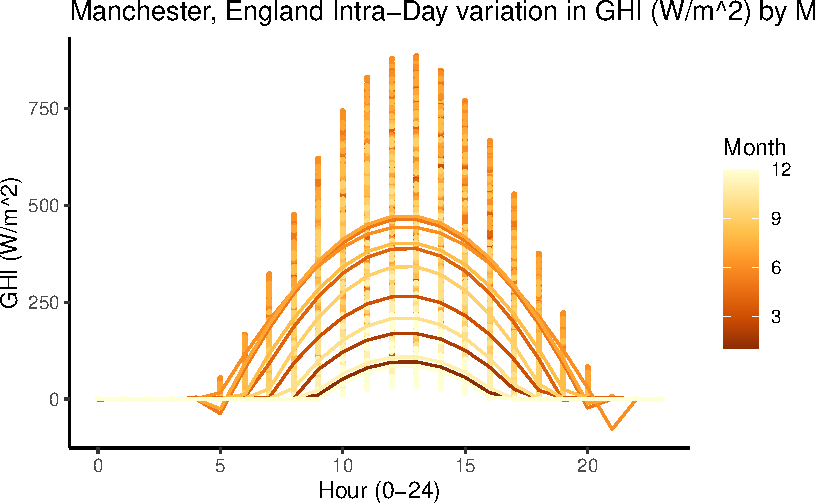
\includegraphics{FinalReport_files/figure-pdf/unnamed-chunk-5-1.pdf}

Compared to both Victoria and Nairobi, Manchester's plot looks less
clean. This is due to the variation in the length of nighttime across
each month, as outlined above. Along the same lines, Manchester has a
wider distribution due to this variation, with days in the summer months
lasting much longer than those in the winter months. Additionally,
Manchester's fitted lines are clustered towards the bottom of the
distribution, whereas Victoria's and Nairobi's are clustered near the
top, indicating the prevalence of low GHI days in Manchester, and high
GHI days in Seychelles and Kenya.

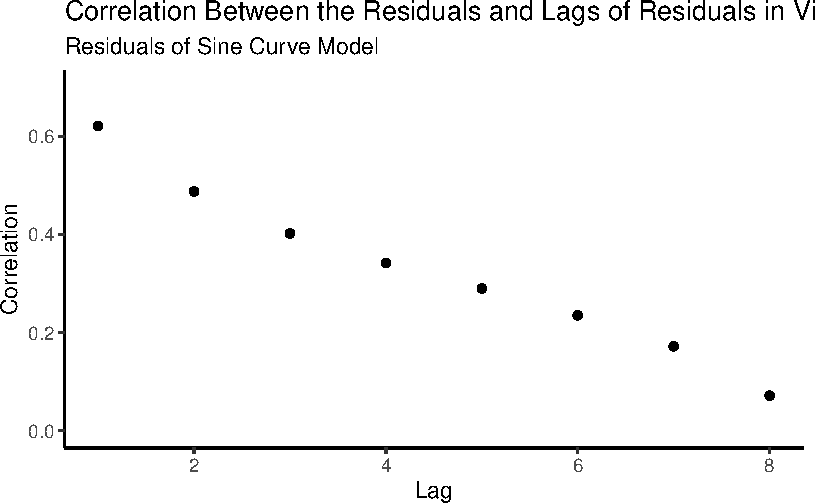
\includegraphics{FinalReport_files/figure-pdf/unnamed-chunk-6-1.pdf}

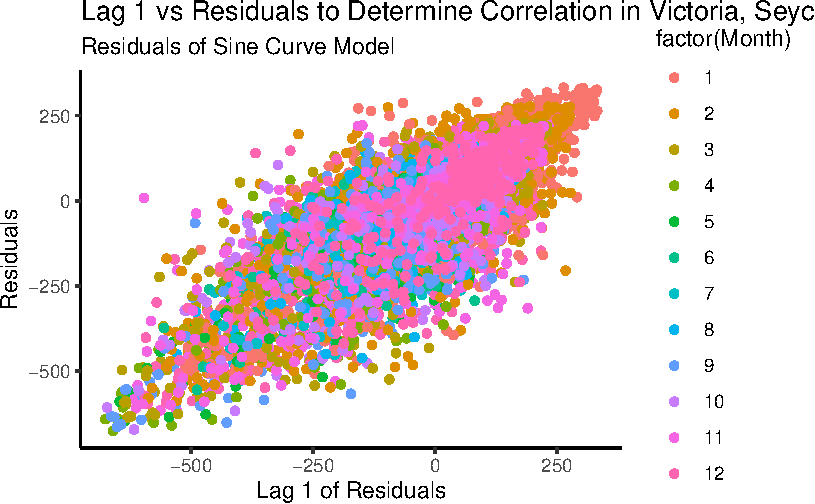
\includegraphics{FinalReport_files/figure-pdf/unnamed-chunk-6-2.pdf}

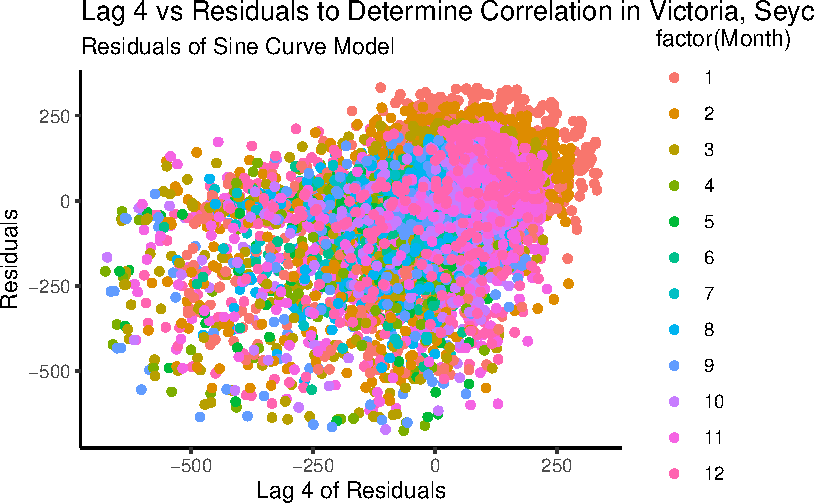
\includegraphics{FinalReport_files/figure-pdf/unnamed-chunk-6-3.pdf}

The final step in using a time series approach to model the intra-day
variation in GHI is to model the correlation between neighboring hours
in the day. We do that by looking at the distribution of our residuals
from our model, which is basically subtracting our model predictions
from the actual values. The next step is to use tools like an
autocorrelation function (ACF) and a partial autocorrelation function
(PACF) to figure out at what lag does the correlation between a given
data point and the lag X (X being what we are trying to find) of that
data point drop to 0. This could help us choose the order of an
autoregressive or moving average model.

Suppose in our PACF we saw correlation drop to 0 at lag 3. Then, we
would be inclined to use an autoregressive model (AR), with an order of
3. We, however, could not use these methods in order to determine what
order AR or MA (moving average) model to use because of the amount of
zeros during the nighttime in our data.

Therefore, we use a longitudinal model called GEE to fit an
autoregressive model. After running the GEE model with a max of 8 lags
as explanatory variables, and the residuals as the response variable,
only the first 4 lags were significant. That is why we used the GEE
model; it allowed us to determine which lags were significant in
predicting the residual, the data point that the lag is connected too.
In essence, it is similar to the PACF as we condition on the intervening
lags. Whichever lag is no longer significant is the same as ``dropping
to 0'' in a PACF. To contextualize this a bit, this is saying that, if
it is 1 in the afternoon, the GHI at 9 in the morning helps to explain
some of the GHI at 1. But, the GHI at 8 in the morning doesn't quite
explain enough of the GHI at 1 for it to be significant enought to
include in our model. From this, an AR(4) model was determined to be the
most optimal for our data. Interestingly, these conclusions are similar
across both Manchester, Nairobi, and Victoria.

All the plots above were done on the first 5 years of data, from
1998-2002. We did this same process outlined above for each 5 year
segment, for a total of 5 times. The sine curve parameter is the only
difference between models across each 5 year period. Shown below is a
plot of change in the sine curve parameter over time, setting the
1998-2002 parameter as a benchmark.

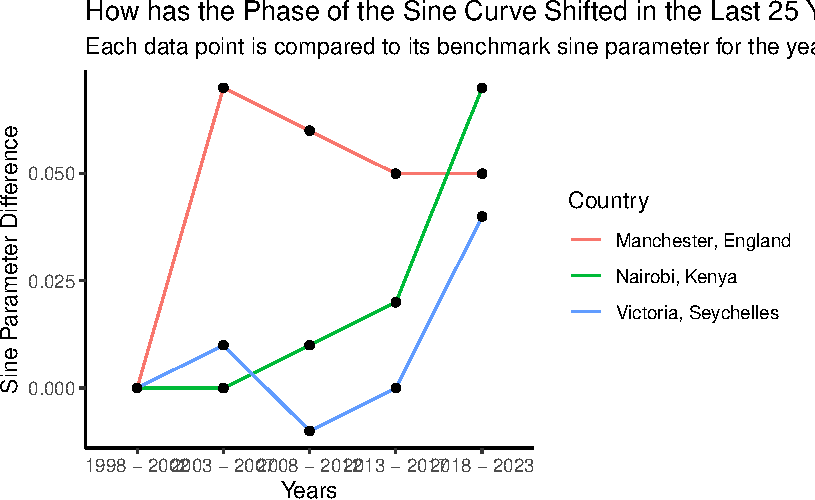
\includegraphics{FinalReport_files/figure-pdf/unnamed-chunk-9-1.pdf}

Interestingly, the phase shift parameter consistently increased from
1998 to 2023 across all 3 locations. Remember that this parameter deals
with the shifting of the sine curve left or right, changing when the
peak of the curve happens in a day. The increase in parameter means
that, from 1998 to 2023, our models' predicted peak of GHI happened
later in the day compared to the 5 year period of 1998 to 2002. This is
an interesting observation, because one might think it be possible for
the amplitude of the sine curve to increase over time, maybe due to
climate change, but where the peak amount of GHI is during the day
should fairly stay the same across time.

Now that we have modeled the intra-day variation in GHI, we next need to
explore the seasonal variation in GHI. How does GHI change throughout a
year?

\hypertarget{seasonal-variation-in-daily-ghi}{%
\subsubsection{Seasonal Variation in Daily
GHI}\label{seasonal-variation-in-daily-ghi}}

Daily GHI data for the Seychelles has multiple sources of seasonality.
The maximum solar energy available changes in a regular pattern because
of the rotation of the earth. Seasonal weather patterns influence the
amount of solar energy reaching the ground (which is available to solar
power installations). Since we have solar insolation data the
seasonality in the maximum energy available is easy to account for. If
we model the maximum GHI for each day of the year based on solar
insolation alone we get a reasonable estimate of maximum GHI.

\begin{figure}

{\centering 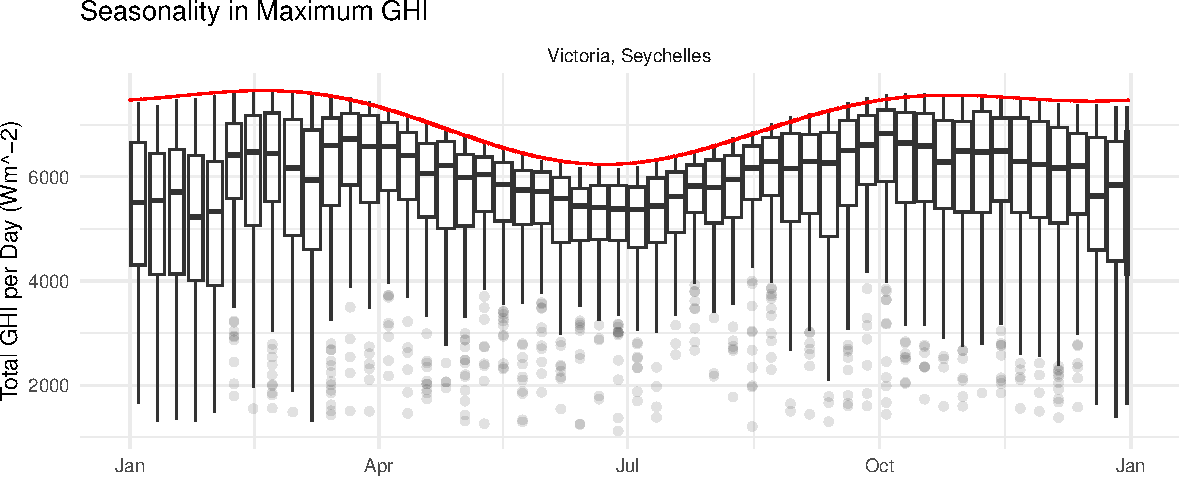
\includegraphics{FinalReport_files/figure-pdf/seychelles ghi-1.pdf}

}

\end{figure}

To deal with the first source of seasonality we change our approach.
Instead of modeling GHI, we examine the fraction of energy that reaches
the ground using the equation:

\[
\text{Fraction of energy reaching ground} = 1 - \frac{\text{Solar Insolation per Day} - \text{GHI per Day}}{\text{Solar Insolation per Day}}
\]

We can now see the effect of seasonal weather patterns more easily. On
average, in clear skies, over the entire earth, the atmosphere reflects
about 30\% of incoming solar energy back into space (Rhodes 2010). In
the graph, we can see that the maximum fraction of solar energy that
reaches the ground is about 70\%. Most days are not perfectly clear
though so typically less than 70\% of the energy reaches the surface.

We estimated the overall trend in the fraction of energy reaching the
surface for each location. Each year we expect the fraction of energy
reaching the ground to fall by 0.00173 and 0.00168 percentage points in
Victoria and Nairobi, respectively, but rise by 0.0008 percentage points
in Manchester. Solar insolation does not change significantly over these
time frames so the trend we observe is likely a result of climate change
and weather.

The seasonality not explained by the seasonality of insolation can also
be explained by climate and weather: Seychelles receives the most
precipitation in January and December, with relatively dry summers
({``Climate Change Knowledge Portal''} 2023). We decided to model this
using a spline with two knots placed to roughly line up with the
seasons, this is plotted in blue below. We add this model to the
existing trend model.

\begin{figure}

{\centering 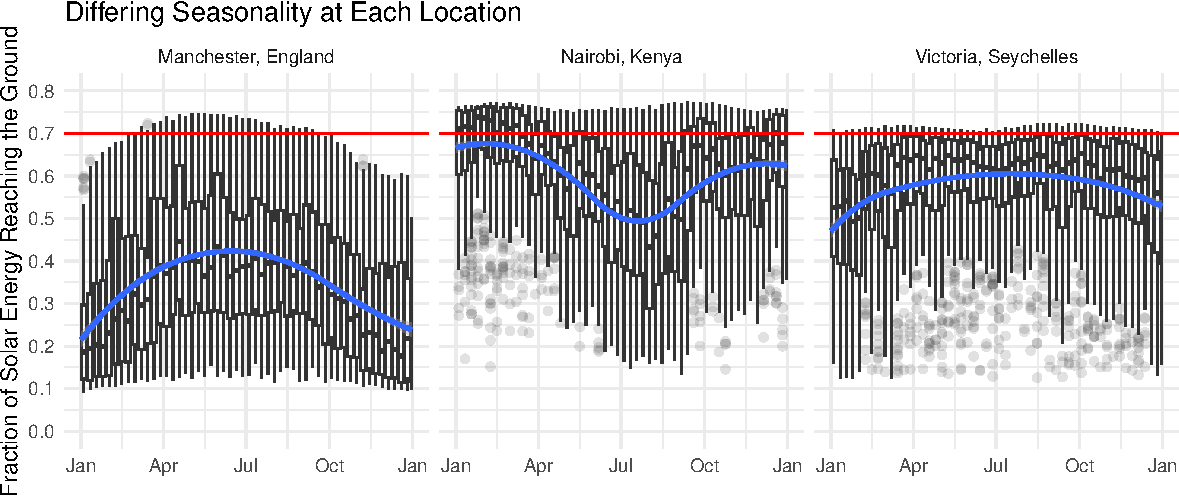
\includegraphics{FinalReport_files/figure-pdf/all energy fraction-1.pdf}

}

\end{figure}

Manchester also sees rainy winters and so exhibits a similar seasonality
({``Climate Change Knowledge Portal''} 2023). In Nairobi, the
seasonality is not associated with precipitation but rather with low
clouds that are present in June, July, and August (Ng'ang'a 1992). This
background on the seasons informs our placement of knots for a spline
model plotted in blue. The residuals of this approach have significant
relationships with humidity, suggesting we should add humidity to our
model.

Average daily relative humidity lets us model more of the relationship
between weather and the energy reaching the ground. Humidity impacts the
clear sky GHI (the GHI if there were no clouds) and can give us some
sense of cloud cover since the data lacks any direct measure of cloud
cover. We incorporate humidity into the three seasonal models as a
degree 1 spline with a single knot. This reflects the observation that
the unexplained relationship with humidity is relatively flat at lower
humidity but is more negative at higher humidity. Kenya and England have
their knots at a relative humidity of 60\%, the Seychelles has its at
75\%. This greatly reduces or eliminates the relationship between the
model residuals and humidity.

\begin{figure}

{\centering 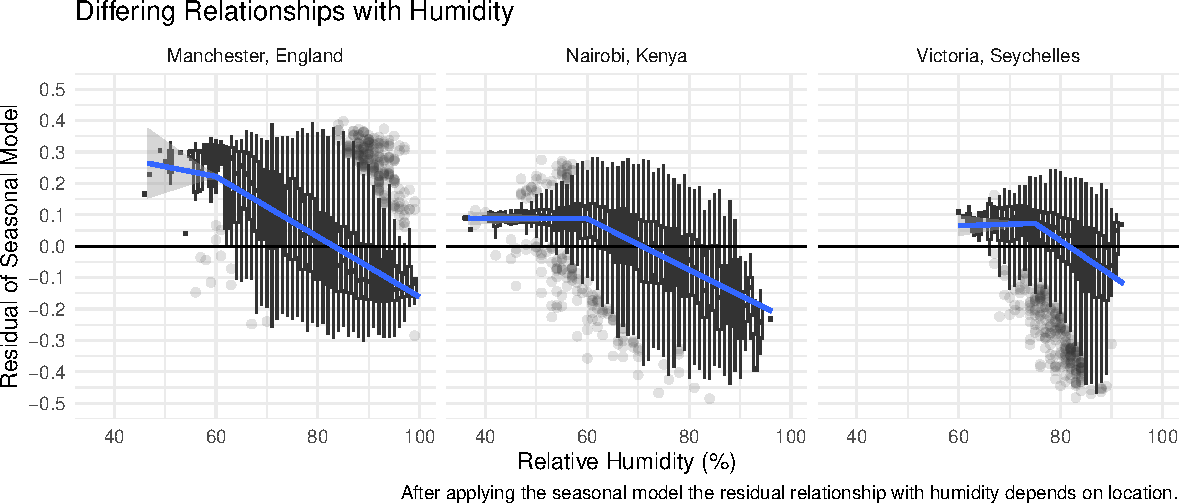
\includegraphics{FinalReport_files/figure-pdf/seasonal residuals-1.pdf}

}

\end{figure}

If we examine just a short period in the Seychelles, the first 2 months
of 2002, it appears that many of the shorter-term fluctuations in GHI
are still present after modeling. These fluctuations seem to be about
2-4 days long which is why the AR models with order 2-4 performed well
on various error metrics.

\begin{figure}

\begin{minipage}[t]{0.50\linewidth}

{\centering 

\raisebox{-\height}{

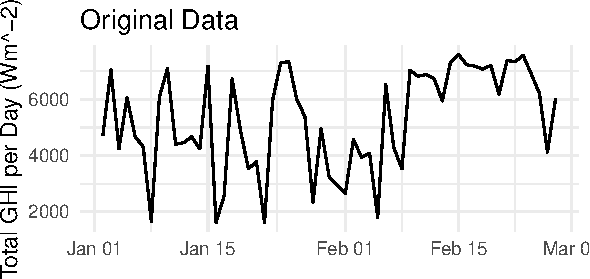
\includegraphics{FinalReport_files/figure-pdf/unnamed-chunk-11-1.pdf}

}

}

\end{minipage}%
%
\begin{minipage}[t]{0.50\linewidth}

{\centering 

\raisebox{-\height}{

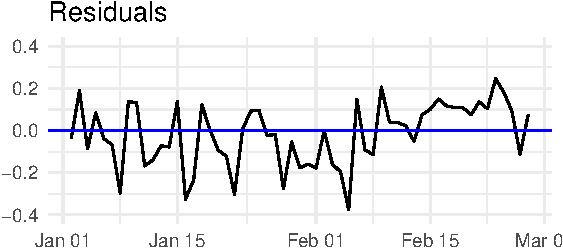
\includegraphics{FinalReport_files/figure-pdf/unnamed-chunk-11-2.pdf}

}

}

\end{minipage}%

\end{figure}

The errors of the combined model with seasonality, humidity, and the
overall trend are not white noise, so we attempt to model them. The ACF
plot tells us the correlation between errors that are a specific number
of lags (measured in days) apart. The ACF decreases as the lags
increase. This makes sense because the farther away two points are from
one another in time, the weaker the correlation between those two values
will be. The PACF plot tells us the correlation between errors and a
specific number of lags apart after accounting for the correlation
between shorter lags. Values within the dashed lines indicate
independent white noise.

\begin{figure}

{\centering 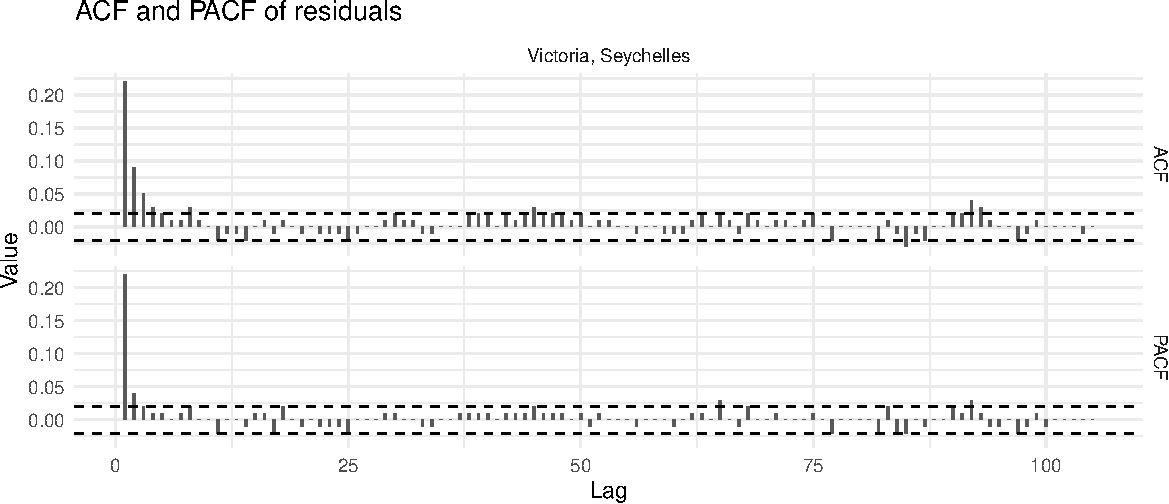
\includegraphics{FinalReport_files/figure-pdf/unnamed-chunk-13-1.pdf}

}

\end{figure}

We come up with five candidate models after looking at the ACF and PACF:
an AR3 model, an AR2 model, an AR2MA1 model, an AR3MA1 model, and an
AR3MA2 model. These choices are primarily based on the slower decay of
the ACF and the PACF being within the dashed lines after 3 lags. Of
these, the AR2MA1 model performs the best as measured by AIC (A goodness
of fit measure with a penalty for model terms). The Ljung-Box statistic
has large p-values, so we fail to reject the null hypothesis that the
residuals are independent There is no proof of serial correlation after
fitting the model. The AR3 model performed very similarly on all metrics
but has slightly worse fit as measured by AIC.

This procedure is repeated for Manchester and Nairobi with similar
results. Using the same criteria as above we settle on an AR3MA1 model
for Manchester and England. In England, the AR4 and AR3 models performed
well. In Kenya, the AR3 model also performed well. The actual effects of
these models are very slight, but they do handle the correlation
present.

\begin{figure}

{\centering 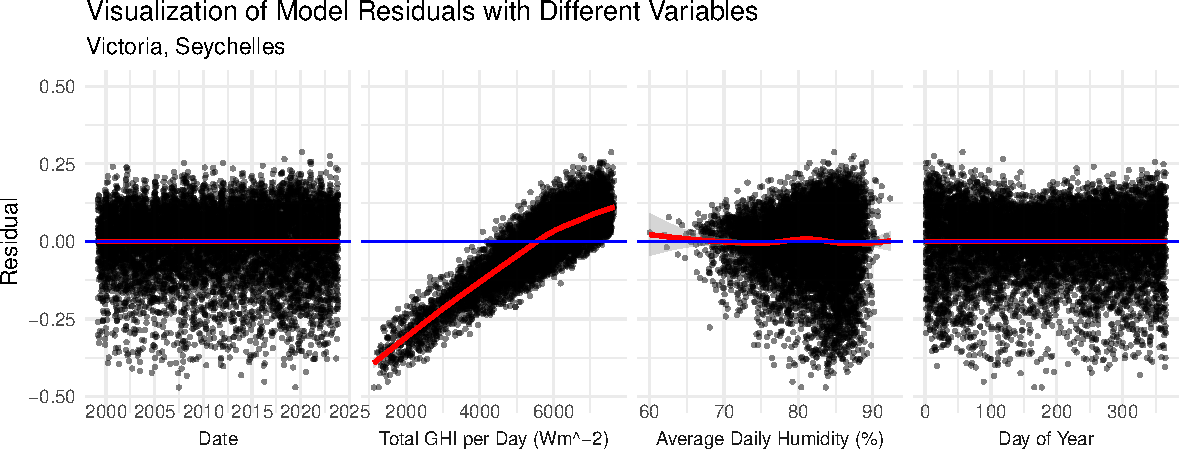
\includegraphics{FinalReport_files/figure-pdf/unnamed-chunk-14-1.pdf}

}

\end{figure}

The Seychelles model residuals have a reasonably insignificant
relationship with date, day of year, and humidity. The strong positive
relationship between daily GHI and the residual suggests a major issue
with the model: we underpredict the fraction of sun reaching the ground
on days with higher total GHI and overpredict on days with lower total
GHI.

Forecasting with this complete model is not possible without a provided
forecast for humidity since we relied on having a known humidity value
when creating the model.

\hypertarget{discussion-and-conclusions}{%
\subsection{Discussion and
Conclusions}\label{discussion-and-conclusions}}

Researchers have explored many different ways to model GHI. These
methods come down to ways to model weather and cloud cover. Researchers
have used an autoregressive spatio-temporal model to model GHI in the
short term (Dambreville et al. 2014). The forecasts resulting from that
model were just 15 minutes to 1 hour. Yang et al. (2015) uses
exponential smoothing to predict cloud cover and, therefore, GHI. Aside
from time series and spatial approaches, neural networks have proven
quite successful at accounting for the highly complex relationships that
impact GHI. Zang et al. (2020) combine two types of neural networks for
spatio-temporal predictions. This, of course, sacrifices
interpretability.

Using a sine curve to model intra-day changes in GHI is a different
approach than those outlined above, and given the tools at our disposal,
a good approach. The sine curve provided a unique way to capture the
distribution of GHI during a day, and did quite well given the almost
simplistic nature of it. The most challenging aspect of the intraday GHI
was handling when it was nighttime. As discussed above, this involved
different approaches to determine what it meant to be nighttime, but
more importantly, proved challenging in uses traditional time series
techniques to remove trend and model the errors. Nairobi and Victoria
both lie on roughly the same latitude, yet the rank of the monthly sine
curves (which month had the highest amplitude) was quite different when
comparing the two. This indicates that weather patterns are
significantly different for Nairobi and Victoria, as well as that there
isn't a whole lot of noticeable difference between months, leading to
the rank of each month to be different than what we would expect given a
traditional seasonal approach. Unsurprisingly, Manchester's GHI was
significantly lower than both Victoria's and Nairobi's. In the winter
months of December and Janurary, the amplitude of the curve was
significantly lower than the corresponding ``winter'' months for
Victoria and Nairobi.

Our approach to modeling the daily sunlight highlights the incredible
variation between different locations and the difficulty of accurately
forecasting weather conditions. When first converting from GHI to our
metric, the fraction of sunlight reaching the ground, each location was
at a different latitude and required a different set of solar insolation
data. This solar insolation data simplifies the modeling process but
there was still a lot to model. The overall trend in the fraction of
sunlight reaching the ground, which has been roughly linear, is also
different for each of the three locations. Each location experienced
different climate and yearly weather patterns and required separate
spline models for the time of year. Even the relationship between
relative humidity and the fraction of sunlight reaching the ground was
unique between the locations. Residuals after all this modeling showed
correlation for data 2 to 4 days apart. That is just a result of how the
weather tends to work from day to day. Each of the locations showed
relatively similar results for this part of the modeling.

The overall trend we saw in daily sunlight in the Seychelles could be a
part of general trends in cloud cover in the Area. Sharma et al. (2023)
shows that cloud cover in the Arabian Sea (north of the Seychelles) has
started to increase and predicts that it will continue to increase as
climate change continues. These results are not generalizable as they
find the opposite trend in the South-East Indian Ocean.

Overall, the model performed poorly. Lacking a solid proxy for cloud
cover in the data, we had little way to predict the day-to-day changes
in cloud cover. Of course, modeling would be very straightforward if we
had a measure of cloud cover. The fraction of sunlight reaching the
ground is directly linked to cloud cover. That would also force us to
rely on some outside cloud cover forecast if we wanted to do any
forecasting. In existing work, spatial data and spatial models play a
critical role. Weather is notoriously difficult to predict and this
difficulty is amplified when the data you have is for single locations
hundreds of miles apart.

\hypertarget{references}{%
\subsection*{References}\label{references}}
\addcontentsline{toc}{subsection}{References}

\hypertarget{refs}{}
\begin{CSLReferences}{1}{0}
\leavevmode\vadjust pre{\hypertarget{ref-boland2020}{}}%
Boland, John. 2020. {``Characterising Seasonality of Solar Radiation and
Solar Farm Output.''} \emph{Energies} 13 (2): 471.
\url{https://doi.org/10.3390/en13020471}.

\leavevmode\vadjust pre{\hypertarget{ref-worldbankclimate}{}}%
{``Climate Change Knowledge Portal.''} 2023. World Bank Group.
\url{https://climateknowledgeportal.worldbank.org/}.

\leavevmode\vadjust pre{\hypertarget{ref-crook2011}{}}%
Crook, Julia A., Laura A. Jones, Piers M. Forster, and Rolf Crook. 2011.
{``Climate Change Impacts on Future Photovoltaic and Concentrated Solar
Power Energy Output.''} \emph{Energy \& Environmental Science} 4 (9):
3101. \url{https://doi.org/10.1039/c1ee01495a}.

\leavevmode\vadjust pre{\hypertarget{ref-dambreville2014}{}}%
Dambreville, Romain, Philippe Blanc, Jocelyn Chanussot, and Didier
Boldo. 2014. {``Very Short Term Forecasting of the Global Horizontal
Irradiance Using a Spatio-Temporal Autoregressive Model.''}
\emph{Renewable Energy} 72 (December): 291--300.
\url{https://doi.org/10.1016/j.renene.2014.07.012}.

\leavevmode\vadjust pre{\hypertarget{ref-insolationdefinition2016}{}}%
Hartmann, Dennis L. 2016. {``The Global Energy Balance.''} In, 25--48.
Elsevier. \url{https://doi.org/10.1016/b978-0-12-328531-7.00002-5}.

\leavevmode\vadjust pre{\hypertarget{ref-databackground2023}{}}%
{``Historical Data Validation.''} 2023. Clean Power Researh;
SolarAnywhere.
\url{https://www.solaranywhere.com/resources/validation/historical/}.

\leavevmode\vadjust pre{\hypertarget{ref-nairobi}{}}%
Ng'ang'a, JK. 1992. {``The Climate and Meteorology of Nairobi Region,
Kenya.''} \emph{Journal Of Social Development In Africa} 7 (1,2).
\url{http://erepository.uonbi.ac.ke:8080/xmlui/handle/123456789/33021}.

\leavevmode\vadjust pre{\hypertarget{ref-rhodes2010}{}}%
Rhodes, Christopher J. 2010. {``Solar Energy: Principles and
Possibilities.''} \emph{Science Progress} 93 (1): 37--112.
\url{https://doi.org/10.3184/003685010x12626410325807}.

\leavevmode\vadjust pre{\hypertarget{ref-climlab2022}{}}%
Rose, Brian, Andrew Williams, Moritz Kreuzer, Chris Cardinale, Sebastian
Meßlinger, Xoviat, Ryan Abernathey, Filipe, and Paul Gierz. 2022.
\emph{Climlab/Climlab: Version 0.8.1}. Zenodo.
\url{https://doi.org/10.5281/ZENODO.6575235}.

\leavevmode\vadjust pre{\hypertarget{ref-shahsavari2018}{}}%
Shahsavari, Amir, and Morteza Akbari. 2018. {``Potential of Solar Energy
in Developing Countries for Reducing Energy-Related Emissions.''}
\emph{Renewable and Sustainable Energy Reviews} 90 (July): 275--91.
\url{https://doi.org/10.1016/j.rser.2018.03.065}.

\leavevmode\vadjust pre{\hypertarget{ref-sharma2023}{}}%
Sharma, Sahil, Kyung-Ja Ha, Ryohei Yamaguchi, Keith B. Rodgers, Axel
Timmermann, and Eui-Seok Chung. 2023. {``Future Indian Ocean Warming
Patterns.''} \emph{Nature Communications} 14 (1).
\url{https://doi.org/10.1038/s41467-023-37435-7}.

\leavevmode\vadjust pre{\hypertarget{ref-GHIbackground2012}{}}%
Stein, Joshua, Clifford Hansen, and Matthew Reno. 2012. {``Global
Horizontal Irradiance Clear Sky Models : Implementation and Analysis.''}
\url{https://doi.org/10.2172/1039404}.

\leavevmode\vadjust pre{\hypertarget{ref-wild2017}{}}%
Wild, Martin, Doris Folini, and Florian Henschel. 2017. {``Impact of
Climate Change on Future Concentrated Solar Power (CSP) Production.''}
\emph{AIP Conference Proceedings}.
\url{https://doi.org/10.1063/1.4975562}.

\leavevmode\vadjust pre{\hypertarget{ref-yang2015}{}}%
Yang, Dazhi, Vishal Sharma, Zhen Ye, Lihong Idris Lim, Lu Zhao, and
Aloysius W. Aryaputera. 2015. {``Forecasting of Global Horizontal
Irradiance by Exponential Smoothing, Using Decompositions.''}
\emph{Energy} 81 (March): 111--19.
\url{https://doi.org/10.1016/j.energy.2014.11.082}.

\leavevmode\vadjust pre{\hypertarget{ref-zang2020}{}}%
Zang, Haixiang, Ling Liu, Li Sun, Lilin Cheng, Zhinong Wei, and Guoqiang
Sun. 2020. {``Short-Term Global Horizontal Irradiance Forecasting Based
on a Hybrid CNN-LSTM Model with Spatiotemporal Correlations.''}
\emph{Renewable Energy} 160 (November): 26--41.
\url{https://doi.org/10.1016/j.renene.2020.05.150}.

\end{CSLReferences}



\end{document}
